\documentclass[a4paper,12pt]{article}

% Добавляем новые пакеты
\usepackage{pifont}
\usepackage{emoji}
\usepackage[russian]{babel}  % Для поддержки русского языка
\usepackage[english, russian]{babel}    % Пакет для поддержки русского языка
\usepackage[T1, T2A]{fontenc}           % Загружаем пакет с поддержкой кирилицы
\usepackage[utf8]{inputenc}             % Загружаем пакет с поддержкой кодировки файла и символов
\usepackage{graphicx}                   % Загружаем пакет для добавления различной графики (pdf, jpg, png)
\usepackage{import}                     % Загружаем пакет для продвинутого импорта, в частности изображений pdf_tex из графического редактора inkscape
\usepackage{subcaption}                 % Пакет для поддержки сетки из фигур, например в две колонки или матрицей
\usepackage{float}        
\usepackage{fontawesome}
% Пакет для улучшенного размещения изображенией
\usepackage{geometry}                   % Пакет для управления отступами на странице
\usepackage{amsmath}                    % Добавляем крутую поддержку математики
\usepackage{amsfonts}                   % Пакет с математическими шрифтами
\usepackage{tabu}                       % Пакет с прокаченными таблицами
\usepackage{booktabs}                   % Крутые вертикальные разделители
\usepackage[dvipsnames]{xcolor}         % Расширенная поддержка цветов
\usepackage[colorlinks]{hyperref}
\usepackage{indentfirst}                % Пакет, чтобы починить красную строку
\usepackage{listings}                   % Поддержка листингов, оформления кода программы
\usepackage{longtable}
\usepackage{makecell}
\usepackage{multirow}
\usepackage{tabularray}
\usepackage{ amssymb }
\usepackage{varwidth}
\usepackage{bm}

\graphicspath{ {./images/} }

% Устанавливает отступы на странице
\geometry{left=2cm, right=2cm, bottom=2cm, top=2cm}

% Настраиваем красивые цвета для ссылок на формулы, фигуры (изображения) и другие элементы.
\hypersetup{
    linkcolor=blue,
    filecolor=magenta,
    urlcolor=cyan
}

% Настраиваем супер красивые листинги
\definecolor{codegreen}{rgb}{0,0.6,0}
\definecolor{codegray}{rgb}{0.5,0.5,0.5}
\definecolor{codepurple}{rgb}{0.58,0,0.82}
\definecolor{backcolour}{rgb}{0.95,0.95,0.92}

\lstdefinestyle{codestyle}{
    backgroundcolor=\color{backcolour},
    commentstyle=\color{codegreen},
    keywordstyle=\color{magenta},
    numberstyle=\tiny\color{codegray},
    stringstyle=\color{codepurple},
    basicstyle=\ttfamily\footnotesize,
    breakatwhitespace=false,
    breaklines=true,
    captionpos=b,
    keepspaces=true,
    numbers=left,
    numbersep=5pt,
    showspaces=false,
    showstringspaces=false,
    showtabs=false,
    tabsize=2
}

\lstset{style=codestyle}
\lstset{extendedchars=\true}

\begin{document}
\begin{titlepage}
    \centering
    \vspace*{1cm}

    {\large Министерство науки и высшего образования Российской Федерации}\\
    {\large ФЕДЕРАЛЬНОЕ ГОСУДАРСТВЕННОЕ АВТОНОМНОЕ ОБРАЗОВАТЕЛЬНОЕ УЧРЕЖДЕНИЕ ВЫСШЕГО ОБРАЗОВАНИЯ «НАЦИОНАЛЬНЫЙ ИССЛЕДОВАТЕЛЬСКИЙ УНИВЕРСИТЕТ ИТМО»}\\
    {\large (УНИВЕРСИТЕТ ИТМО)}\\

    \vspace{2cm}

    {\large Факультет «Систем управления и робототехники»}\\

    \vspace{3cm}

    \textbf{{\Huge ОТЧЕТ}\\
    {\Huge О ЛАБОРАТОРНОЙ РАБОТЕ №1}}\\

    \vspace{1cm}

    {\LARGE По дисциплине «Техническое зрение»}\\
    {\LARGE на тему: «Гистограммы, профили и проекции»}\\

    \vspace{3cm}

    {\Large Студент:}\\
    Охрименко Ева ИСУ 409290\\


    \vspace{2cm}

    {\Large Проверил:}\\
   Шаветов Сергей Васильевич\\

    \vspace{4cm}

    {\large г. Санкт-Петербург}\\
    {\large 2024}

\end{titlepage}

\tableofcontents  % Оглавление
\newpage
\section{Task. Гистограммы}

\subsection{Функция \texttt{plot\_histograms}. Построение гистограмм}

Функция строит гистограммы для исходного изображения.

\subsubsection{Код}
\begin{verbatim}
def plot_histograms(original, transformed, title):
    colors = ('b', 'g', 'r')
    plt.figure(figsize=(14, 6))
    
    plt.subplot(2, 2, 1)
    for i, color in enumerate(colors):
        hist = cv2.calcHist([original], [i], None, [256], [0, 256])
        hist = hist / (original.shape[0] * original.shape[1])
        plt.plot(hist, color=color)
        plt.xlim([0, 256])
    plt.title("Гистограмма исходного изображения")
    plt.xlabel('Интенсивность пикселей')
    plt.ylabel('Плотность пикселей')
\end{verbatim}

\subsubsection{Объяснение}
Функция принимает исходное и преобразованное изображения, а также заголовок. Для каждого канала (B, G, R) вычисляется гистограмма с помощью \texttt{cv2.calcHist}. Гистограмма нормируется на общее количество пикселей, после чего строится график. Добавляются подписи осей и заголовок.

\subsubsection{Итог}
На вход подаются исходное и преобразованное изображения. На выходе получается график гистограммы исходного изображения.

\subsubsection{Выход}

\begin{figure}[H]
    \centering
    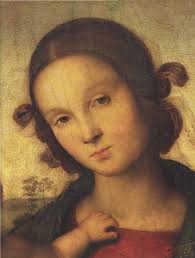
\includegraphics[width=0.3\textwidth]{im/im.jpg}
    \caption{Исходное изображение}
    \label{fig:example_image}
\end{figure}
\begin{figure}[H]
    \centering
    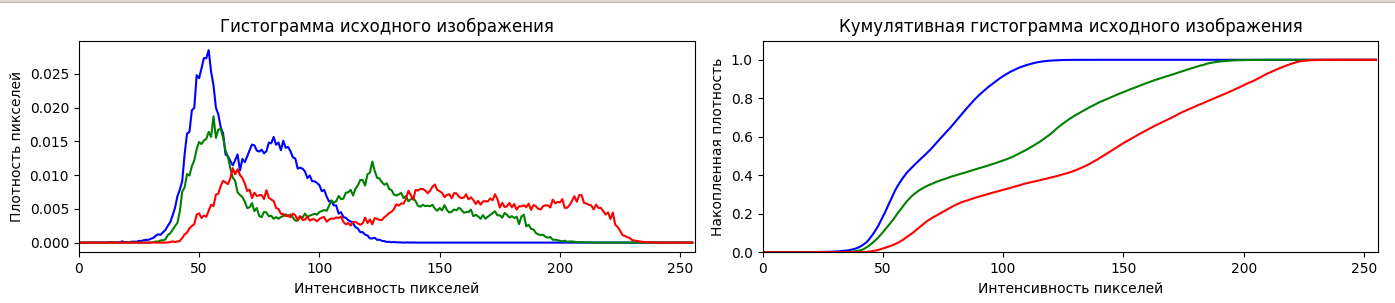
\includegraphics[width=1.0\textwidth]{im/1.png}
    \caption{Гистограмма исходного изображения}
    \label{fig:example_image}
\end{figure}



\subsection{Функция \texttt{uniform\_transform}. Равномерное преобразование}

Функция растягивает интенсивности изображения на весь диапазон [0, 1] или [0, 255].

\subsubsection{Код}
\begin{verbatim}
def uniform_transform(I):
    Inew = I.astype(np.float32) / 255 if I.dtype == np.uint8 else I
    Imin, Imax = Inew.min(), Inew.max()
    Inew = (Inew - Imin) / (Imax - Imin)
    return (Inew * 255).clip(0, 255).astype(np.uint8) if I.dtype == np.uint8 else Inew
\end{verbatim}

\subsubsection{Объяснение}
Функция принимает изображение и выполняет растяжение динамического диапазона. Если изображение в формате \texttt{uint8}, оно нормализуется в диапазон [0, 1]. Затем находятся минимальное (\texttt{Imin}) и максимальное (\texttt{Imax}) значения интенсивности. Интенсивности растягиваются на весь диапазон [0, 1] с помощью формулы:
\[
\text{Inew} = \frac{\text{Inew} - \text{Imin}}{\text{Imax} - \text{Imin}}.
\]
Если исходное изображение было в формате \texttt{uint8}, результат преобразуется обратно в этот формат.

\subsubsection{Итог}
На вход подается изображение. На выходе получается изображение с улучшенным контрастом, где интенсивности растянуты на весь доступный диапазон.

\subsubsection{Выход}

\begin{figure}[H]
    \centering
    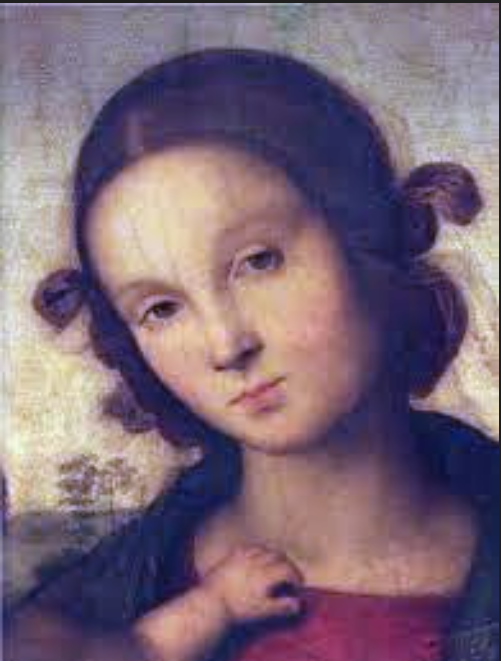
\includegraphics[width=0.3\textwidth]{im/imРастяжение.png}
    \caption{Полученное изображение после равномерного преобразования}
    \label{fig:uniform_image}
\end{figure}

\begin{figure}[H]
    \centering
    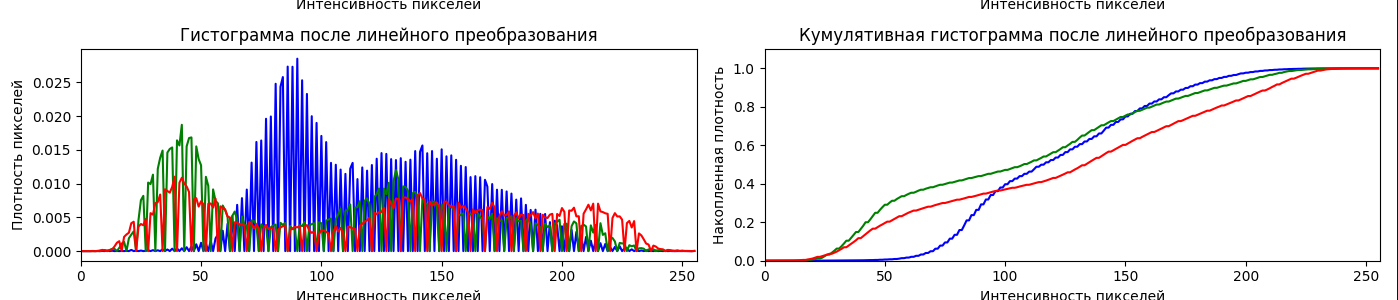
\includegraphics[width=1\textwidth]{im/гистограммаРастяжение.png}
    \caption{Гистограмма после равномерного преобразования}
    \label{fig:uniform_histogram}
\end{figure}



\subsection{Функция \texttt{arithmetic\_operations}. Арифметические операции}

Функция увеличивает яркость изображения на заданное значение.

\subsubsection{Код}
\begin{verbatim}
def arithmetic_operations(I, value=50):
    Inew = I.astype(np.float32) + value / 255
    Inew = np.clip(Inew, 0, 1)
    if I.dtype == np.uint8:
        Inew = (255 * Inew).clip(0, 255).astype(np.uint8)
    return Inew
\end{verbatim}

\subsubsection{Объяснение}
Функция принимает изображение и значение \texttt{value}, на которое увеличивается яркость. Изображение преобразуется в формат \texttt{float32}, и к его интенсивностям добавляется значение \texttt{value / 255}. Результат обрезается до диапазона [0, 1]. Если исходное изображение было в формате \texttt{uint8}, результат преобразуется обратно в этот формат.

\subsubsection{Итог}
На вход подается изображение и значение \texttt{value}. На выходе получается изображение с увеличенной яркостью. Если исходное изображение было в формате \texttt{uint8}, результат также будет в этом формате.

\subsubsection{Выход}

\begin{figure}[H]
    \centering
    
\includegraphics[width=0.3\textwidth]{im/imАрифметика.png}
    \caption{Полученное изображение после арифметической операции}
    \label{fig:arithmetic_image}
\end{figure}

\begin{figure}[H]
    \centering
    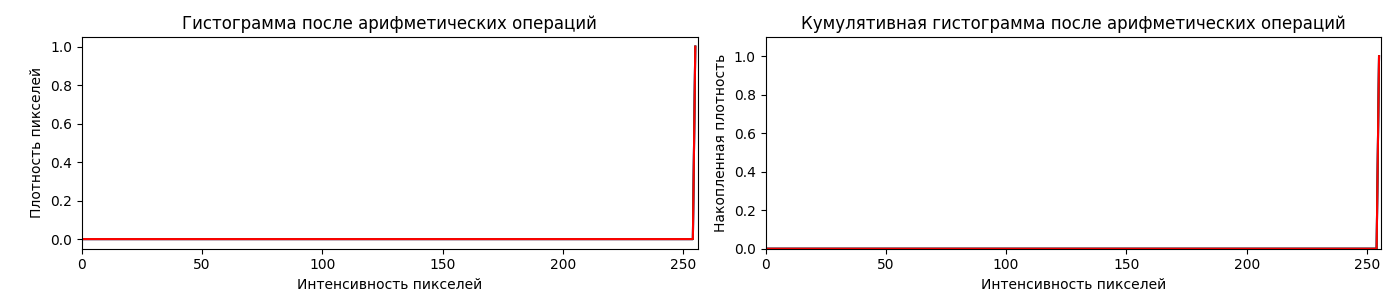
\includegraphics[width=1\textwidth]{im/гистограммаАрифметика.png}
    \caption{Гистограмма после арифметической операции}
    \label{fig:arithmetic_histogram}
\end{figure}



\subsection{Функция \texttt{dynamic\_range\_stretching}. Растяжение динамического диапазона}

Функция выполняет растяжение динамического диапазона изображения, улучшая его контраст.

\subsubsection{Код}
\begin{verbatim}
def dynamic_range_stretching(I):
    if I.dtype == np.uint8:
        Inew = I.astype(np.float32) / 255
    else:
        Inew = I
    
    I_BGR = cv2.split(Inew)
    Inew_BGR = []
    
    for layer in I_BGR:
        Imin = layer.min()
        Imax = layer.max()
        Inew_layer = (layer - Imin) / (Imax - Imin)
        Inew_BGR.append(Inew_layer)
    
    Inew = cv2.merge(Inew_BGR)
    if I.dtype == np.uint8:
        Inew = (255 * Inew).clip(0, 255).astype(np.uint8)
    
    return Inew
\end{verbatim}

\subsubsection{Объяснение}
Функция принимает изображение и выполняет растяжение динамического диапазона для каждого канала (B, G, R). Если изображение в формате \texttt{uint8}, оно нормализуется в диапазон [0, 1]. Для каждого канала находятся минимальное (\texttt{Imin}) и максимальное (\texttt{Imax}) значения интенсивности, после чего интенсивности растягиваются на весь диапазон [0, 1] с помощью формулы:
\[
\text{Inew\_layer} = \frac{\text{layer} - \text{Imin}}{\text{Imax} - \text{Imin}}.
\]
Преобразованные каналы объединяются обратно в одно изображение.

\subsubsection{Итог}
На вход подается изображение. На выходе получается изображение с улучшенным контрастом, где интенсивности каждого канала растянуты на весь диапазон [0, 1].


\subsubsection{Выход}

\begin{figure}[H]
    \centering
    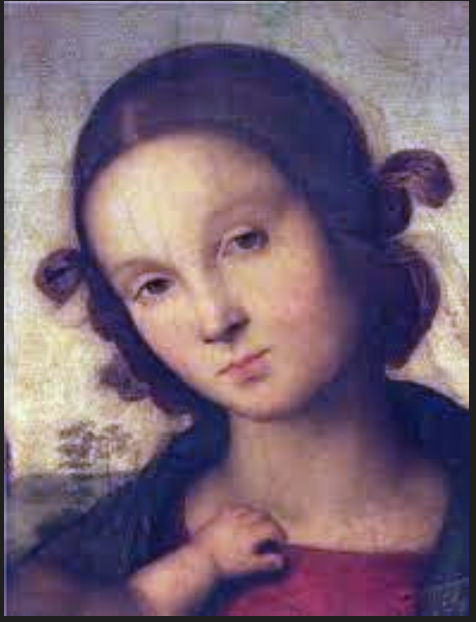
\includegraphics[width=0.3\textwidth]{im/imРастяжениеДиапазона.png}
    \caption{Полученное изображение}
    \label{fig:example_image}
\end{figure}
\begin{figure}[H]
    \centering
    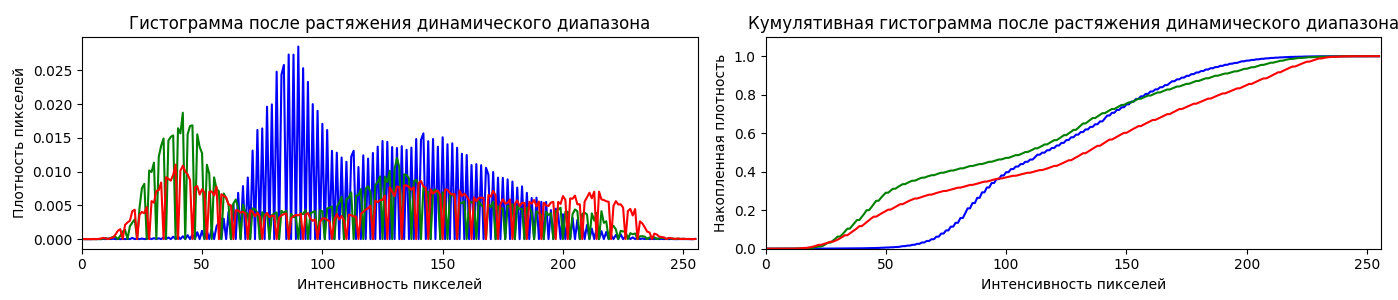
\includegraphics[width=1\textwidth]{im/4.png}
    \caption{Гистограмма после растяжения диапазона}
    \label{fig:example_image}
\end{figure}


\subsection{Функция \texttt{exponential\_transform}. Экспоненциальное преобразование}

Функция применяет экспоненциальное преобразование к изображению с параметром \( \alpha \).

\subsubsection{Код}
\begin{verbatim}
def exponential_transform(I, alpha=1.0):
    if I.dtype == np.uint8:
        Inew = I.astype(np.float32) / 255
    else:
        Inew = I

    Imin = Inew.min()

    Inew = Imin - (1 / alpha) * np.log(1 - Inew)
    
    Inew = np.clip(Inew, 0, 1)
    
    if I.dtype == np.uint8:
        Inew = (255 * Inew).clip(0, 255).astype(np.uint8)
    
    return Inew
\end{verbatim}

\subsubsection{Объяснение}
Функция принимает изображение и параметр \( \alpha \), который определяет форму экспоненциального преобразования. Если изображение в формате \texttt{uint8}, оно нормализуется в диапазон [0, 1]. Затем находится минимальное значение интенсивности (\texttt{Imin}). К изображению применяется экспоненциальное преобразование:
\[
\text{Inew} = \text{Imin} - \frac{1}{\alpha} \cdot \ln(1 - \text{Inew}).
\]
Результат обрезается до диапазона [0, 1]. Если исходное изображение было в формате \texttt{uint8}, результат преобразуется обратно в этот формат.

\subsubsection{Итог}
На вход подается изображение и параметр \( \alpha \). На выходе получается изображение, к которому применено экспоненциальное преобразование. Если исходное изображение было в формате \texttt{uint8}, результат также будет в этом формате.

\subsubsection{Выход}

\begin{figure}[H]
    \centering
    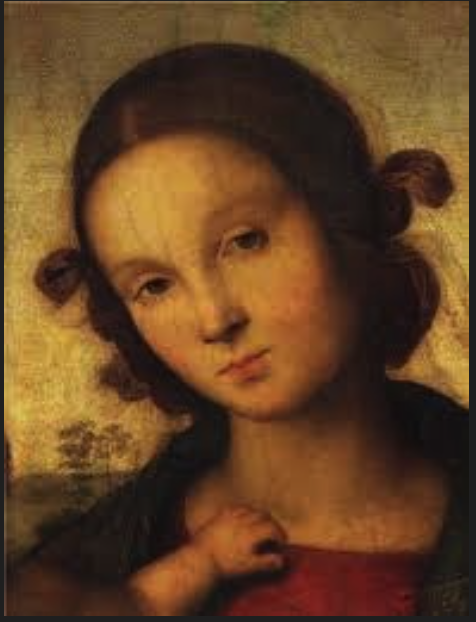
\includegraphics[width=0.3\textwidth]{im/imЭкспонента.png}
    \caption{Полученное изображение после экспоненциального преобразования}
    \label{fig:exponential_image}
\end{figure}

\begin{figure}[H]
    \centering
    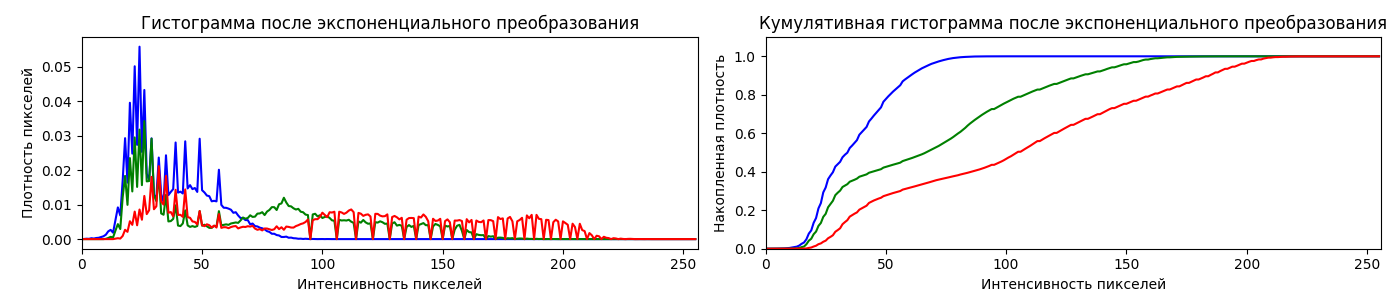
\includegraphics[width=1\textwidth]{im/гистограммаЭкспонента.png}
    \caption{Гистограмма после экспоненциального преобразования}
    \label{fig:exponential_histogram}
\end{figure}




\subsection{Функция \texttt{rayleigh\_transform}. Преобразование по закону Рэлея}

Функция применяет преобразование интенсивности изображения по закону Рэлея с параметром \( \alpha \).

\subsubsection{Код}
\begin{verbatim}
def rayleigh_transform(I, alpha=1.0):
    if I.dtype == np.uint8:
        Inew = I.astype(np.float32) / 255
    else:
        Inew = I

    Imin = Inew.min()

    Inew = Imin + np.sqrt(2 * alpha**2 * np.log(1 / (1 - Inew)))

    Inew = np.clip(Inew, 0, 1)

    if I.dtype == np.uint8:
        Inew = (255 * Inew).clip(0, 255).astype(np.uint8)
    
    return Inew
\end{verbatim}

\subsubsection{Объяснение}
Функция принимает изображение и параметр \( \alpha \), который определяет форму распределения Рэлея. Если изображение в формате \texttt{uint8}, оно нормализуется в диапазон [0, 1]. Затем находится минимальное значение интенсивности (\texttt{Imin}). К изображению применяется преобразование по закону Рэлея:
\[
\text{Inew} = \text{Imin} + \sqrt{2 \alpha^2 \ln\left(\frac{1}{1 - \text{Inew}}\right)}.
\]
Результат обрезается до диапазона [0, 1]. Если исходное изображение было в формате \texttt{uint8}, результат преобразуется обратно в этот формат.

\subsubsection{Итог}
На вход подается изображение и параметр \( \alpha \). На выходе получается изображение, к которому применено преобразование по закону Рэлея. Если исходное изображение было в формате \texttt{uint8}, результат также будет в этом формате.

\subsubsection{Выход}

\begin{figure}[H]
    \centering
    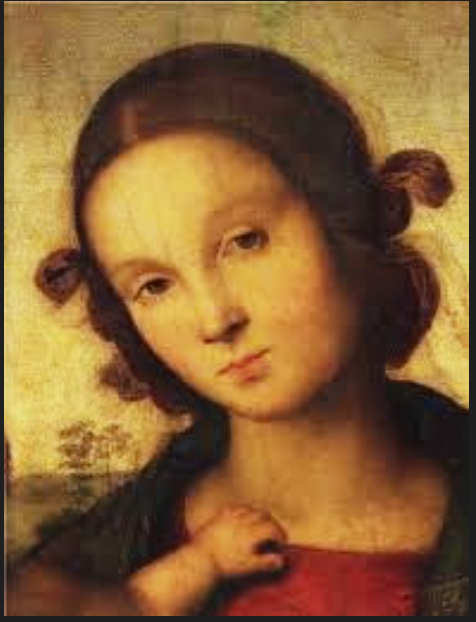
\includegraphics[width=0.3\textwidth]{im/imРелея.png}
    \caption{Полученное изображение после преобразования Рэлея}
    \label{fig:rayleigh_image}
\end{figure}

\begin{figure}[H]
    \centering
    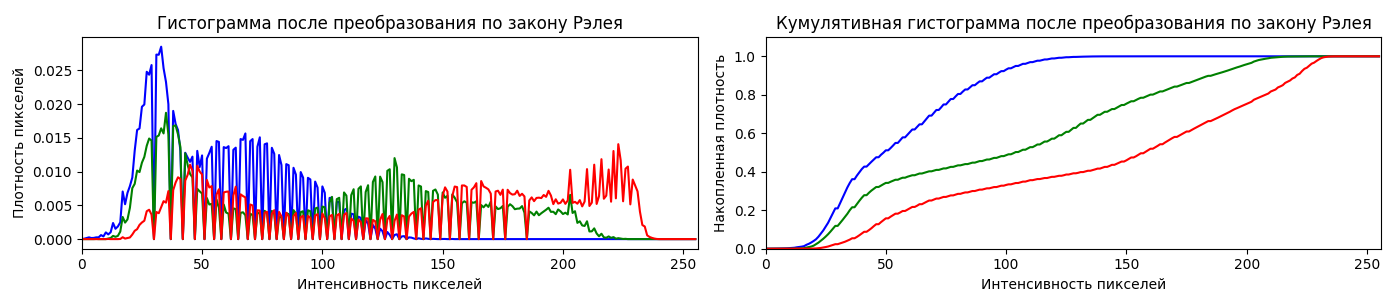
\includegraphics[width=1\textwidth]{im/гистограммаРелея.png}
    \caption{Гистограмма после преобразования Рэлея}
    \label{fig:rayleigh_histogram}
\end{figure}




\subsection{Функция \texttt{power\_law\_transform}. Степенное преобразование}

Функция применяет степенное преобразование к изображению с показателем степени \( \frac{2}{3} \).

\subsubsection{Код}
\begin{verbatim}
def power_law_transform(I):
    if I.dtype == np.uint8:
        Inew = I.astype(np.float32) / 255
    else:
        Inew = I
    
    Inew = np.power(Inew, 2/3)
    Inew = np.clip(Inew, 0, 1)
    
    if I.dtype == np.uint8:
        Inew = (255 * Inew).clip(0, 255).astype(np.uint8)
    
    return Inew
\end{verbatim}

\subsubsection{Объяснение}
Функция принимает изображение и применяет к нему степенное преобразование с показателем степени \( \frac{2}{3} \). Если изображение в формате \texttt{uint8}, оно нормализуется в диапазон [0, 1]. Затем к изображению применяется преобразование:
\[
\text{Inew} = \text{Inew}^{\frac{2}{3}}.
\]
Результат обрезается до диапазона [0, 1]. Если исходное изображение было в формате \texttt{uint8}, результат преобразуется обратно в этот формат.

\subsubsection{Итог}
На вход подается изображение. На выходе получается изображение, к которому применено степенное преобразование с показателем степени \( \frac{2}{3} \). Если исходное изображение было в формате \texttt{uint8}, результат также будет в этом формате.

\subsubsection{Выход}

\begin{figure}[H]
    \centering
    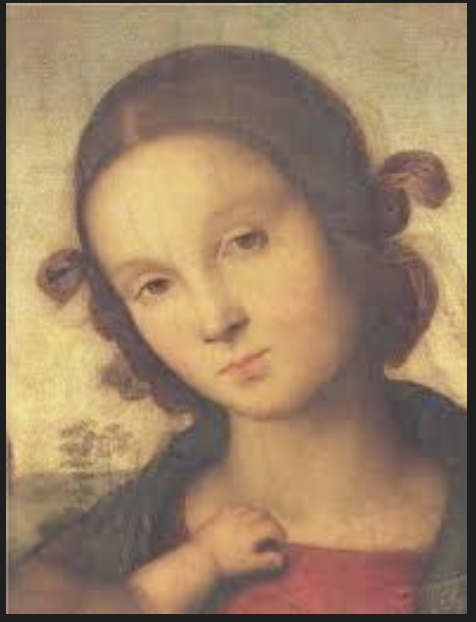
\includegraphics[width=0.3\textwidth]{im/imСтепенное.png}
    \caption{Полученное изображение после степенного преобразования}
    \label{fig:power_law_image}
\end{figure}

\begin{figure}[H]
    \centering
    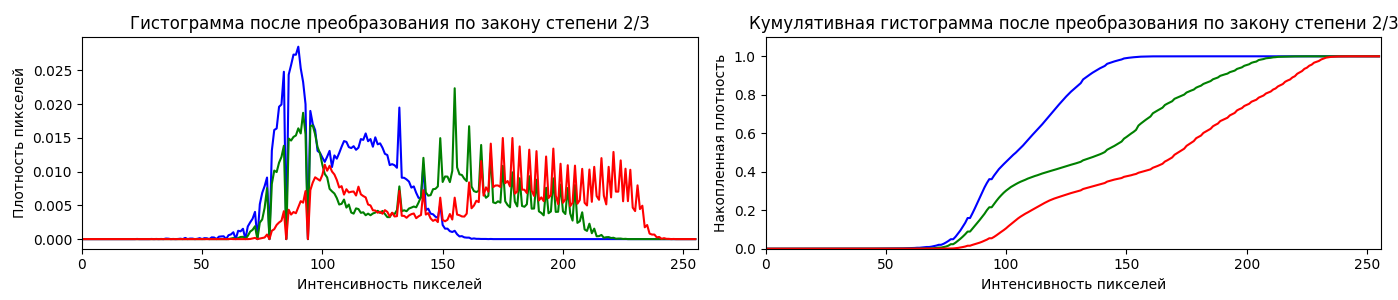
\includegraphics[width=1\textwidth]{im/гистограммаСтепенное.png}
    \caption{Гистограмма после степенного преобразования}
    \label{fig:power_law_histogram}
\end{figure}


\subsection{Функция \texttt{hyperbolic\_transform}. Гиперболическое преобразование}

Функция применяет гиперболическое преобразование к изображению с параметром \( \alpha \).

\subsubsection{Код}
\begin{verbatim}
def hyperbolic_transform(I, alpha=2.0):
    if I.dtype == np.uint8:
        P_I = I.astype(np.float32) / 255
    else:
        P_I = I

    Inew = np.power(alpha, P_I)

    Inew = np.clip(Inew, 0, 1)

    if I.dtype == np.uint8:
        Inew = (255 * Inew).clip(0, 255).astype(np.uint8)
    
    return Inew
\end{verbatim}

\subsubsection{Объяснение}
Функция принимает изображение и параметр \( \alpha \), который определяет основание гиперболического преобразования. Если изображение в формате \texttt{uint8}, оно нормализуется в диапазон [0, 1]. Затем к изображению применяется гиперболическое преобразование:
\[
\text{Inew} = \alpha^{\text{P\_I}}.
\]
Результат обрезается до диапазона [0, 1]. Если исходное изображение было в формате \texttt{uint8}, результат преобразуется обратно в этот формат.

\subsubsection{Итог}
На вход подается изображение и параметр \( \alpha \). На выходе получается изображение, к которому применено гиперболическое преобразование. Если исходное изображение было в формате \texttt{uint8}, результат также будет в этом формате.

\subsubsection{Выход}

\begin{figure}[H]
    \centering
    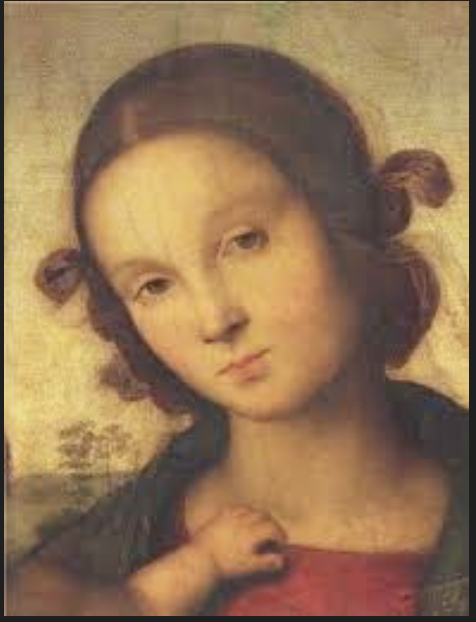
\includegraphics[width=0.3\textwidth]{im/imГиперболическое.png}
    \caption{Полученное изображение после гиперболического преобразования}
    \label{fig:hyperbolic_image}
\end{figure}

\begin{figure}[H]
    \centering
        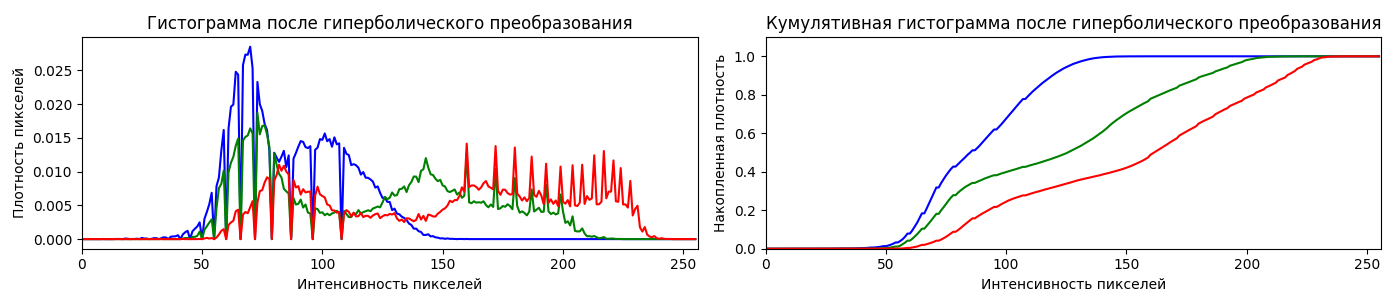
\includegraphics[width=1\textwidth]{im/гистограммаГиперболическое.png}
    \caption{Гистограмма после гиперболического преобразования}
    \label{fig:hyperbolic_histogram}
\end{figure}


\subsection{Вывод}

В этом задании я разобралась с разными методами улучшения изображений и реализовала их на практике. Каждый метод я протестировала на слабоконтрастной картинке , а результаты визуализировала с помощью гистограмм. Вот что у меня получилось:

\subsubsection{Арифметические операции}
С помощью арифметических операций можно легко увеличить яркость изображения. Это особенно полезно, если картинка слишком темная. Метод простой и быстрый, поэтому его удобно использовать для базовой обработки.

\subsubsection{Растяжение динамического диапазона}
Этот метод отлично подходит для изображений, где яркости сосредоточены в узком диапазоне. Он растягивает их на весь доступный диапазон, делая картинку более выразительной. 

\subsubsection{Равномерное преобразование}
Равномерное преобразование помогает растянуть яркости на весь диапазон, что особенно полезно для картинок с плохим контрастом. В результате изображение становится более детализированным и приятным для глаз.

\subsubsection{Экспоненциальное преобразование}
Экспоненциальное преобразование позволяет гибко настраивать контраст с помощью параметра \( \alpha \). Этот метод особенно полезен, если на изображении есть пересвеченные или слишком темные участки.

\subsubsection{Преобразование по закону Рэлея}
Этот метод хорошо справляется с изображениями, где есть шумы или неравномерное освещение. Параметр \( \alpha \) помогает адаптировать преобразование под конкретные задачи, улучшая видимость деталей в сложных условиях.

\subsubsection{Преобразование по закону степени 2/3}
Степенное преобразование с показателем \( \frac{2}{3} \) улучшает видимость деталей в тенях и средних тонах. Метод прост в реализации и показывает хорошие результаты для большинства изображений.

\subsubsection{Гиперболическое преобразование}
Гиперболическое преобразование усиливает контраст в темных областях изображения. Параметр \( \alpha \) позволяет гибко настраивать результат, что делает метод универсальным для разных задач.


\section{Task. Профили}

\subsection{Функция \texttt{plot\_brightness\_profile}. Построение профиля яркости}

Функция строит график изменения яркости вдоль заданной линии на изображении.

\subsubsection{Код}
\begin{verbatim}
def plot_brightness_profile(image, line_start, line_end):
    height, width = image.shape[:2]
    
    num_points = 1000
    x = np.linspace(line_start[0], line_end[0], num_points)
    y = np.linspace(line_start[1], line_end[1], num_points)

    profile = [image[int(y[i]), int(x[i])] for i in range(num_points)]

    plt.figure(figsize=(8, 4))
    plt.plot(profile, color='black')
    plt.title("Профиль яркости")
    plt.xlabel("Позиция вдоль линии")
    plt.ylabel("Яркость")
    plt.grid(True)
    plt.tight_layout()
    plt.show()
\end{verbatim}

\subsubsection{Объяснение}
Функция принимает изображение и координаты начальной (\texttt{line\_start}) и конечной (\texttt{line\_end}) точек линии. Для построения профиля яркости:
\begin{itemize}
    \item Создается массив точек вдоль линии с использованием \texttt{np.linspace}.
    \item Для каждой точки извлекается значение яркости из изображения.
    \item Строится график изменения яркости вдоль линии.
\end{itemize}

\subsubsection{Итог}
На вход подается изображение и координаты линии. На выходе получается график изменения яркости вдоль этой линии.

\subsubsection{Выход}


\begin{figure}[H]
    \centering
    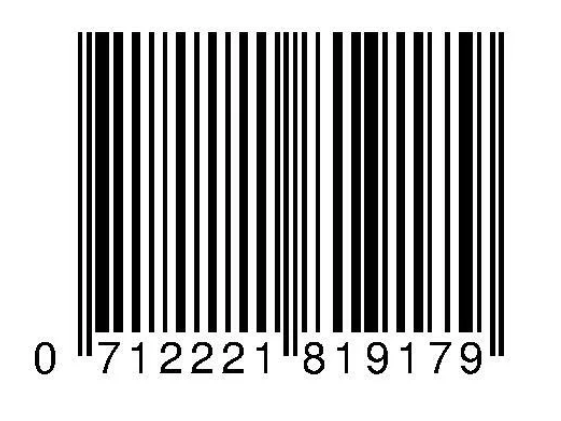
\includegraphics[width=0.5\textwidth]{im/imШтрих.png}
    \caption{Штрих код}
    \label{fig:brightness_profile}
\end{figure}

\begin{figure}[H]
    \centering
    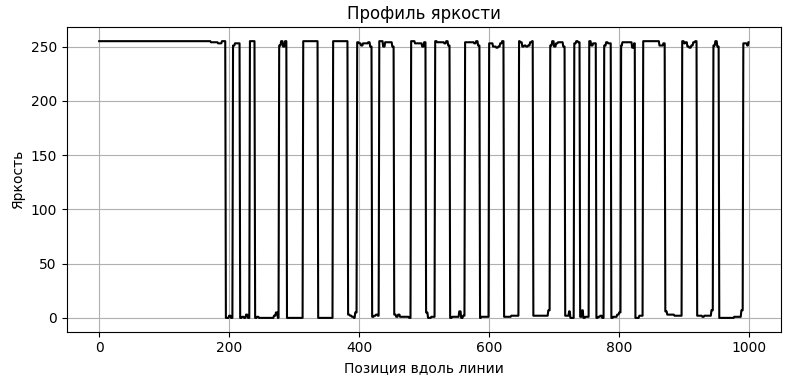
\includegraphics[width=1\textwidth]{im/imПрофильЯркости.png}
    \caption{График профиля яркости}
    \label{fig:brightness_profile}
\end{figure}















\section{Task. Проекции}

\subsection{Функция \texttt{render\_projections}. Построение проекций изображения}

Функция строит проекции изображения на горизонтальную (X) и вертикальную (Y) оси, а также визуализирует исходное изображение.

\subsubsection{Код}
\begin{verbatim}
def render_projections(img):
    gray_img = cv2.cvtColor(img, cv2.COLOR_BGR2GRAY)
    projection_x = np.sum(gray_img, axis=0) / gray_img.shape[0]
    projection_y = np.sum(gray_img, axis=1) / gray_img.shape[1]

    plt.figure(figsize=(12, 6))

    plt.subplot(2, 2, 1)
    plt.title("Исходное изображение")
    plt.imshow(cv2.cvtColor(img, cv2.COLOR_BGR2RGB))
    plt.axis('off')

    plt.subplot(2, 2, 2)
    plt.title("Проекция на X")
    plt.plot(projection_x, color='blue')
    plt.xlabel("Позиция по X")
    plt.ylabel("Интенсивность")
    plt.grid(True)

    plt.subplot(2, 2, 3)
    plt.title("Проекция на Y")
    plt.plot(projection_y, range(gray_img.shape[0]), color='red')
    plt.xlabel("Интенсивность")
    plt.ylabel("Позиция по Y")
    plt.grid(True)

    plt.tight_layout()
    plt.show()
\end{verbatim}

\subsubsection{Объяснение}
Функция принимает цветное изображение и выполняет следующие шаги:
\begin{itemize}
    \item Преобразует изображение в灰度 (оттенки серого) с помощью \texttt{cv2.cvtColor}.
    \item Вычисляет проекцию на горизонтальную ось (X) как сумму интенсивностей по строкам, нормированную на высоту изображения:
    \[
    \text{projection\_x} = \frac{\sum_{\text{строка}} \text{пиксель}}{\text{высота}}.
    \]
    \item Вычисляет проекцию на вертикальную ось (Y) как сумму интенсивностей по столбцам, нормированную на ширину изображения:
    \[
    \text{projection\_y} = \frac{\sum_{\text{столбец}} \text{пиксель}}{\text{ширина}}.
    \]
    \item Визуализирует исходное изображение и графики проекций на X и Y.
\end{itemize}

\subsubsection{Итог}
На вход подается цветное изображение. На выходе получается визуализация исходного изображения и графиков проекций на горизонтальную и вертикальную оси.

\subsubsection{Выход}

\begin{figure}[H]
    \centering
    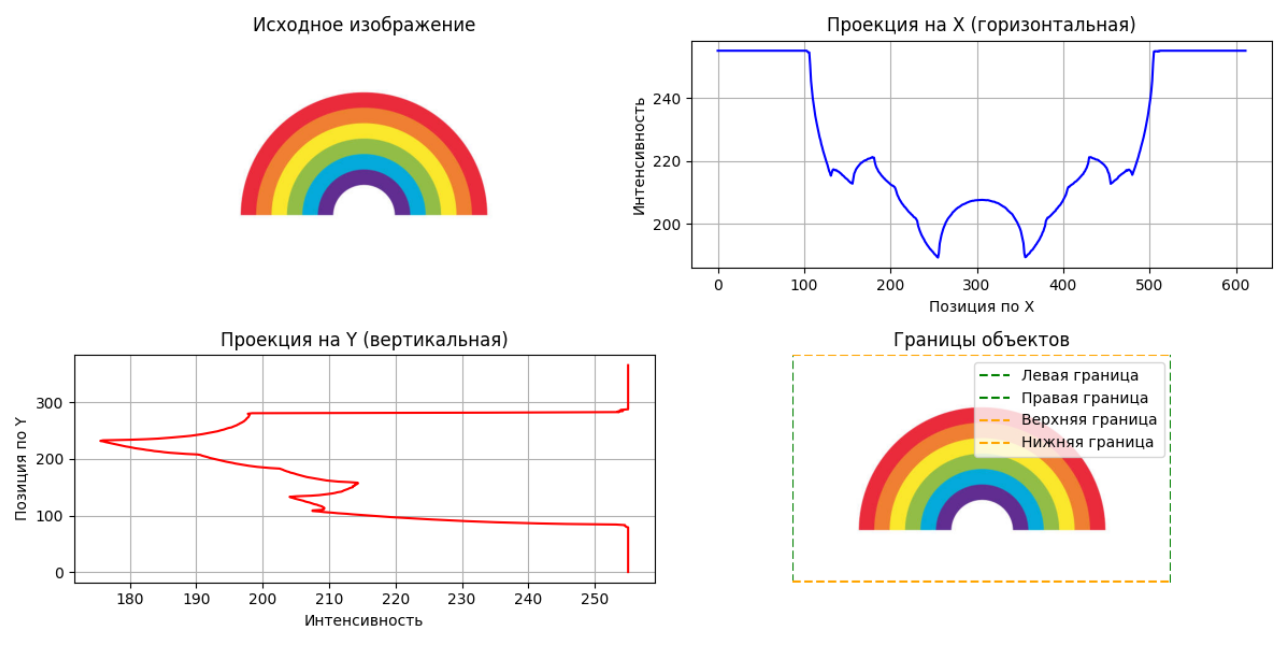
\includegraphics[width=1\textwidth]{im/imПроекции.png}
    \caption{Исходное изображение и проекции на оси X и Y}
    \label{fig:projections}
\end{figure}



\section{Вывод}
В ходе выполнения лабораторной работы я освоила различные методы преобразования изображений для улучшения их визуального качества и упрощения последующего анализа. Я также изучила работу с профилями и проекциями изображений, что позволило мне эффективно выделять границы и объекты на изображениях.

Для реализации задач я использовала библиотеки OpenCV и Matplotlib, которые значительно упростили процесс обработки и визуализации изображений. Эти инструменты помогли мне лучше понять принципы работы различных преобразований и их влияние на изображения.

Скоро все результаты, включая код для генерации гистограмм и других данных, будут доступны в моем репозитории на GitHub \href{https://github.com/decadeos/texViz}{https://github.com/decadeos/texViz}.





\end{document}
